\documentclass{standalone}
\usepackage{tikz}
\usetikzlibrary{patterns, positioning}
\usepackage[sfdefault]{ClearSans} %% option 'sfdefault' activates Clear Sans as the default text font
\usepackage[T1]{fontenc}

\begin{document}
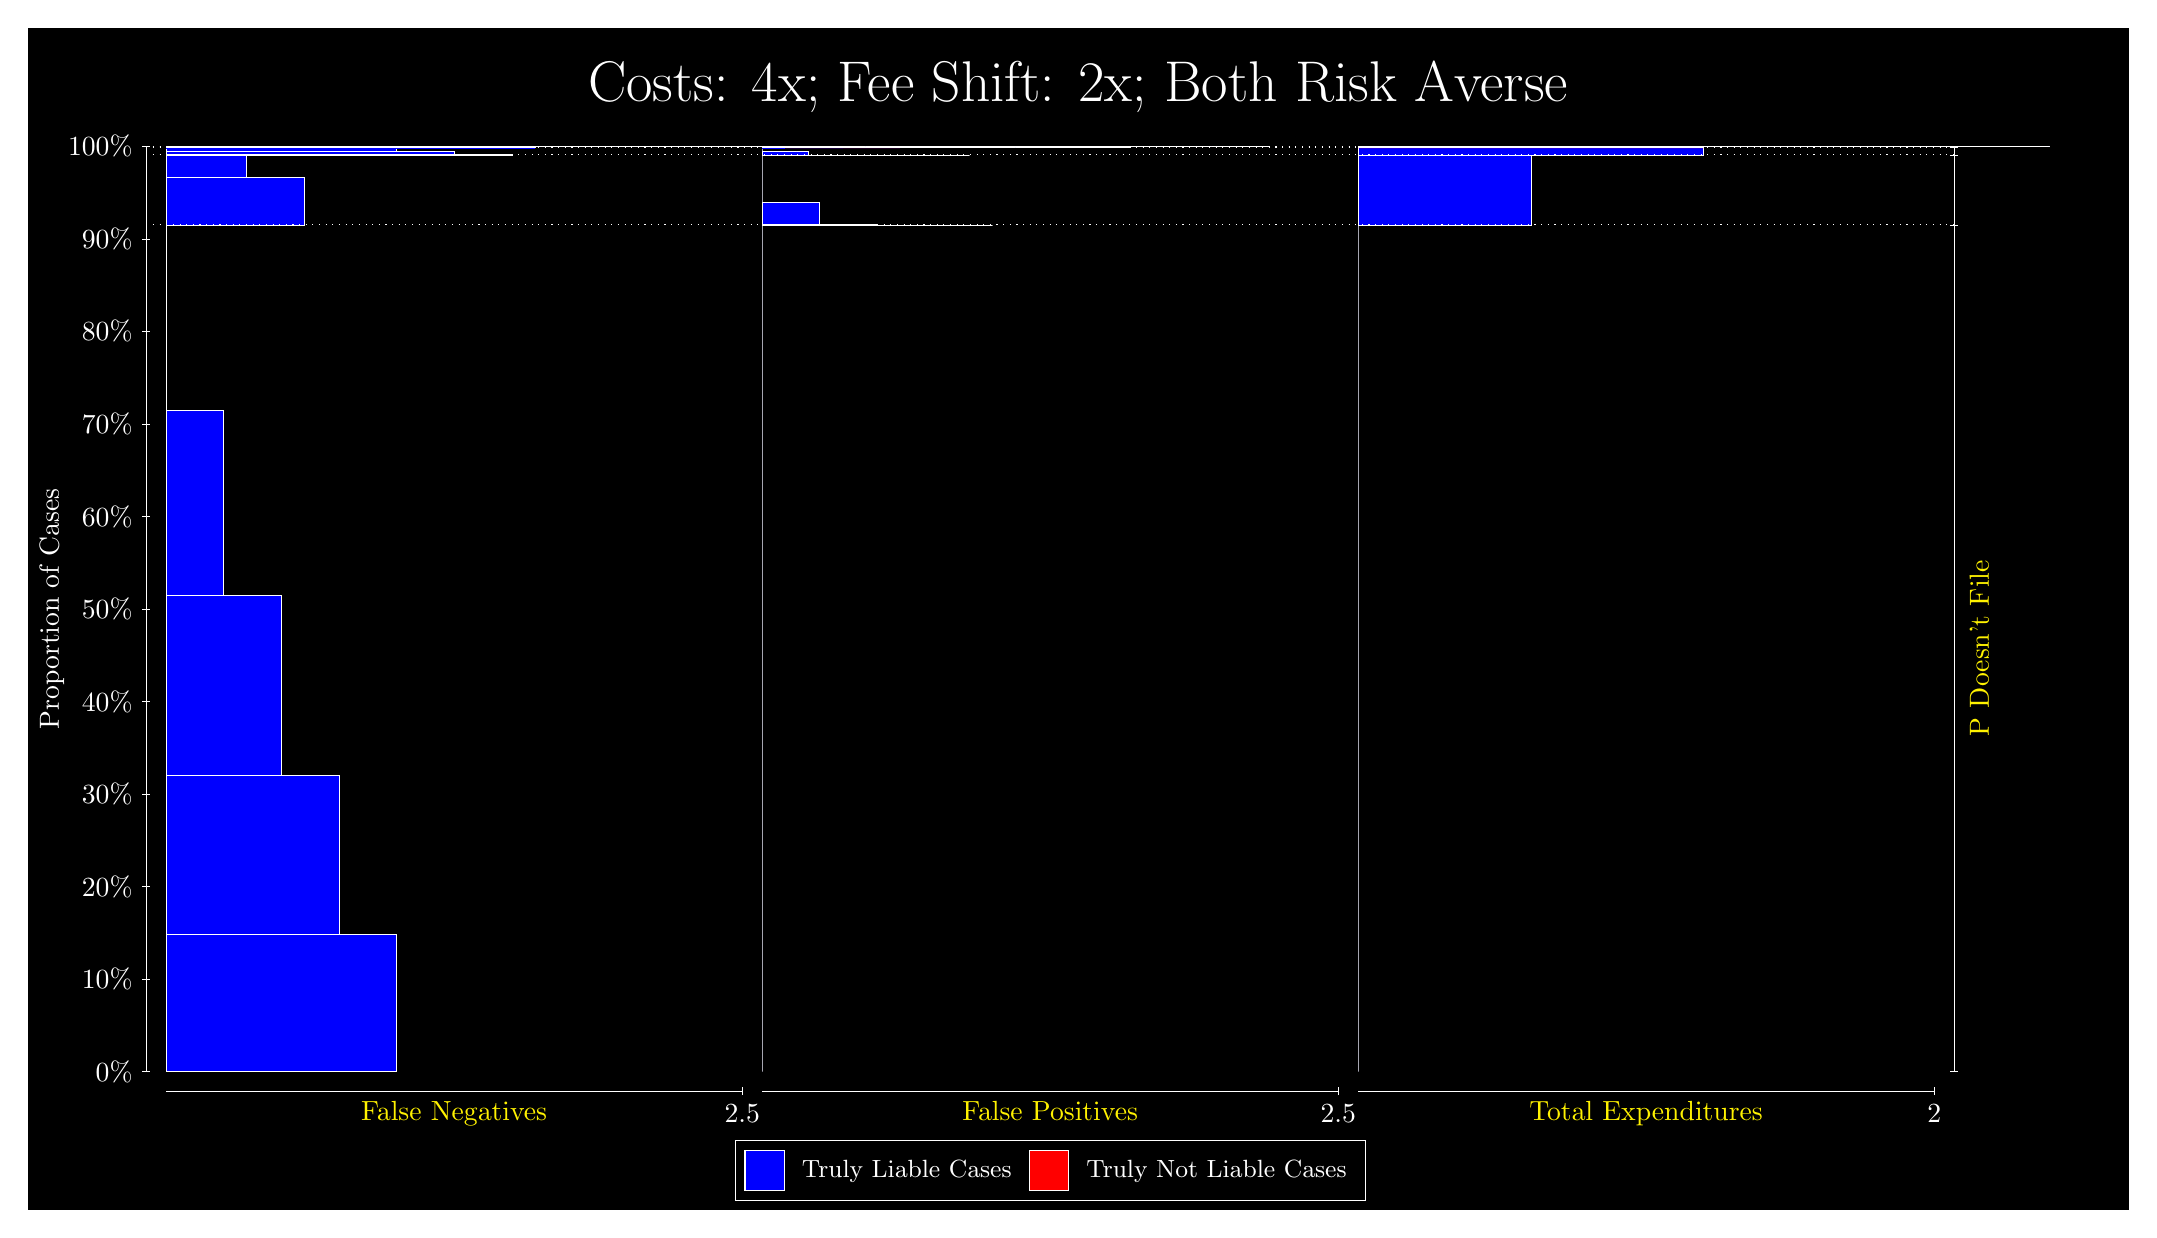
\begin{tikzpicture}
\draw[fill=black] (0,0) rectangle (26.667,15);
\draw[text=white] (0,13.5) rectangle (26.667,15) node[midway] {\huge Costs: 4x; Fee Shift: 2x; Both Risk Averse};
\draw[white, very thin] (1.5,1.75) -- (1.5,13.5);
\node[rotate=90, text=white, anchor=center] at (0.3, 7.625) {Proportion of Cases};
\draw[white, very thin] (1.45,1.75) -- (1.55,1.75);
\node[text=white, anchor=east] at (1.45, 1.75) {0\%};
\draw[white, very thin] (1.45,2.925) -- (1.55,2.925);
\node[text=white, anchor=east] at (1.45, 2.925) {10\%};
\draw[white, very thin] (1.45,4.1) -- (1.55,4.1);
\node[text=white, anchor=east] at (1.45, 4.1) {20\%};
\draw[white, very thin] (1.45,5.275) -- (1.55,5.275);
\node[text=white, anchor=east] at (1.45, 5.275) {30\%};
\draw[white, very thin] (1.45,6.45) -- (1.55,6.45);
\node[text=white, anchor=east] at (1.45, 6.45) {40\%};
\draw[white, very thin] (1.45,7.625) -- (1.55,7.625);
\node[text=white, anchor=east] at (1.45, 7.625) {50\%};
\draw[white, very thin] (1.45,8.8) -- (1.55,8.8);
\node[text=white, anchor=east] at (1.45, 8.8) {60\%};
\draw[white, very thin] (1.45,9.975) -- (1.55,9.975);
\node[text=white, anchor=east] at (1.45, 9.975) {70\%};
\draw[white, very thin] (1.45,11.15) -- (1.55,11.15);
\node[text=white, anchor=east] at (1.45, 11.15) {80\%};
\draw[white, very thin] (1.45,12.325) -- (1.55,12.325);
\node[text=white, anchor=east] at (1.45, 12.325) {90\%};
\draw[white, very thin] (1.45,13.5) -- (1.55,13.5);
\node[text=white, anchor=east] at (1.45, 13.5) {100\%};

\draw[white, very thin] (24.457,1.75) -- (24.457,13.5);
\draw[white, very thin] (24.407,1.75) -- (24.507,1.75);
\node[anchor=west] at (24.407, 1.75) {};
\draw[white, very thin] (24.407,12.503) -- (24.507,12.503);
\node[anchor=west] at (24.407, 12.503) {};
\draw[white, very thin] (24.407,13.391) -- (24.507,13.391);
\node[anchor=west] at (24.407, 13.391) {};
\draw[white, very thin] (24.407,13.484) -- (24.507,13.484);
\node[anchor=west] at (24.407, 13.484) {};
\draw[white, very thin] (24.407,13.493) -- (24.507,13.493);
\node[anchor=west] at (24.407, 13.493) {};
\draw[white, very thin] (24.407,13.498) -- (24.507,13.498);
\node[anchor=west] at (24.407, 13.498) {};
\draw[white, very thin] (24.407,13.5) -- (24.507,13.5);
\node[anchor=west] at (24.407, 13.5) {};

\draw[white, very thin, fill=blue] (1.75,1.75) rectangle (4.6775,3.4924);
\draw[white, very thin, fill=blue] (1.75,3.4924) rectangle (3.9457,5.5071);
\draw[white, very thin, fill=blue] (1.75,5.5071) rectangle (3.2138,7.8034);
\draw[white, very thin, fill=blue] (1.75,7.8034) rectangle (2.4819,10.153);
\draw[white, very thin, fill=red] (1.75,10.153) rectangle (1.75,10.153);
\draw[white, very thin, fill=blue] (1.75,10.153) rectangle (1.75,12.503);
\draw[white, very thin, fill=blue] (1.75,12.503) rectangle (3.5065,13.102);
\draw[white, very thin, fill=blue] (1.75,13.102) rectangle (2.7746,13.382);
\draw[white, very thin, fill=blue] (1.75,13.382) rectangle (2.0428,13.391);
\draw[white, very thin, fill=red] (1.75,13.391) rectangle (1.75,13.391);
\draw[white, very thin, fill=blue] (1.75,13.391) rectangle (1.75,13.391);
\draw[white, very thin, fill=blue] (1.75,13.391) rectangle (6.1413,13.397);
\draw[white, very thin, fill=blue] (1.75,13.397) rectangle (5.8486,13.397);
\draw[white, very thin, fill=blue] (1.75,13.397) rectangle (5.5558,13.397);
\draw[white, very thin, fill=blue] (1.75,13.397) rectangle (5.4094,13.439);
\draw[white, very thin, fill=blue] (1.75,13.439) rectangle (5.1167,13.44);
\draw[white, very thin, fill=blue] (1.75,13.44) rectangle (4.8239,13.44);
\draw[white, very thin, fill=blue] (1.75,13.44) rectangle (4.6775,13.483);
\draw[white, very thin, fill=blue] (1.75,13.483) rectangle (4.3848,13.483);
\draw[white, very thin, fill=blue] (1.75,13.483) rectangle (4.092,13.483);
\draw[white, very thin, fill=blue] (1.75,13.483) rectangle (3.9457,13.484);
\draw[white, very thin, fill=blue] (1.75,13.484) rectangle (3.6529,13.484);
\draw[white, very thin, fill=blue] (1.75,13.484) rectangle (3.3602,13.484);
\draw[white, very thin, fill=blue] (1.75,13.484) rectangle (3.2138,13.484);
\draw[white, very thin, fill=blue] (1.75,13.484) rectangle (2.921,13.484);
\draw[white, very thin, fill=blue] (1.75,13.484) rectangle (2.6283,13.484);
\draw[white, very thin, fill=red] (1.75,13.484) rectangle (1.75,13.484);
\draw[white, very thin, fill=blue] (1.75,13.484) rectangle (6.4341,13.485);
\draw[white, very thin, fill=blue] (1.75,13.485) rectangle (5.7022,13.492);
\draw[white, very thin, fill=blue] (1.75,13.492) rectangle (4.9703,13.493);
\draw[white, very thin, fill=blue] (1.75,13.493) rectangle (4.2384,13.493);
\draw[white, very thin, fill=blue] (1.75,13.493) rectangle (3.5065,13.493);
\draw[white, very thin, fill=red] (1.75,13.493) rectangle (1.75,13.493);
\draw[white, very thin, fill=blue] (1.75,13.493) rectangle (3.5065,13.494);
\draw[white, very thin, fill=blue] (1.75,13.494) rectangle (2.7746,13.497);
\draw[white, very thin, fill=blue] (1.75,13.497) rectangle (2.0428,13.498);
\draw[white, very thin, fill=red] (1.75,13.498) rectangle (1.75,13.498);
\draw[white, very thin, fill=blue] (1.75,13.498) rectangle (1.75,13.498);
\draw[white, very thin, fill=blue] (1.75,13.498) rectangle (15.217,13.498);
\draw[white, very thin, fill=blue] (1.75,13.498) rectangle (14.485,13.498);
\draw[white, very thin, fill=blue] (1.75,13.498) rectangle (13.753,13.498);
\draw[white, very thin, fill=blue] (1.75,13.498) rectangle (13.021,13.498);
\draw[white, very thin, fill=blue] (1.75,13.498) rectangle (12.289,13.498);
\draw[white, very thin, fill=blue] (1.75,13.498) rectangle (7.4587,13.498);
\draw[white, very thin, fill=blue] (1.75,13.498) rectangle (6.7268,13.498);
\draw[white, very thin, fill=blue] (1.75,13.498) rectangle (5.9949,13.498);
\draw[white, very thin, fill=blue] (1.75,13.498) rectangle (5.2631,13.499);
\draw[white, very thin, fill=blue] (1.75,13.499) rectangle (4.5312,13.5);
\draw[white, very thin, fill=blue] (1.75,13.5) rectangle (3.7993,13.5);
\draw[white, very thin, fill=blue] (1.75,13.5) rectangle (3.0674,13.5);
\draw[white, very thin, fill=blue] (1.75,13.5) rectangle (2.3355,13.5);
\draw[white, very thin, fill=red] (1.75,13.5) rectangle (1.75,13.5);
\draw[white, very thin, fill=red] (9.3189,1.75) rectangle (9.3189,1.75);
\draw[white, very thin, fill=blue] (9.3189,1.75) rectangle (9.3189,12.503);
\draw[white, very thin, fill=red] (9.3189,12.503) rectangle (12.246,12.503);
\draw[white, very thin, fill=blue] (9.3189,12.503) rectangle (12.246,12.503);
\draw[white, very thin, fill=blue] (9.3189,12.503) rectangle (11.515,12.503);
\draw[white, very thin, fill=blue] (9.3189,12.503) rectangle (10.783,12.511);
\draw[white, very thin, fill=blue] (9.3189,12.511) rectangle (10.051,12.792);
\draw[white, very thin, fill=blue] (9.3189,12.792) rectangle (9.3189,13.391);
\draw[white, very thin, fill=red] (9.3189,13.391) rectangle (11.954,13.391);
\draw[white, very thin, fill=blue] (9.3189,13.391) rectangle (11.954,13.391);
\draw[white, very thin, fill=red] (9.3189,13.391) rectangle (11.661,13.391);
\draw[white, very thin, fill=blue] (9.3189,13.391) rectangle (11.661,13.391);
\draw[white, very thin, fill=red] (9.3189,13.391) rectangle (11.368,13.391);
\draw[white, very thin, fill=blue] (9.3189,13.391) rectangle (11.368,13.391);
\draw[white, very thin, fill=blue] (9.3189,13.391) rectangle (11.222,13.391);
\draw[white, very thin, fill=blue] (9.3189,13.391) rectangle (10.929,13.391);
\draw[white, very thin, fill=blue] (9.3189,13.391) rectangle (10.636,13.391);
\draw[white, very thin, fill=blue] (9.3189,13.391) rectangle (10.49,13.391);
\draw[white, very thin, fill=blue] (9.3189,13.391) rectangle (10.197,13.391);
\draw[white, very thin, fill=blue] (9.3189,13.391) rectangle (9.9044,13.435);
\draw[white, very thin, fill=blue] (9.3189,13.435) rectangle (9.758,13.435);
\draw[white, very thin, fill=blue] (9.3189,13.435) rectangle (9.4652,13.436);
\draw[white, very thin, fill=blue] (9.3189,13.436) rectangle (9.3189,13.484);
\draw[white, very thin, fill=red] (9.3189,13.484) rectangle (11.075,13.484);
\draw[white, very thin, fill=blue] (9.3189,13.484) rectangle (11.075,13.484);
\draw[white, very thin, fill=blue] (9.3189,13.484) rectangle (10.344,13.484);
\draw[white, very thin, fill=blue] (9.3189,13.484) rectangle (9.6116,13.485);
\draw[white, very thin, fill=blue] (9.3189,13.485) rectangle (9.3189,13.493);
\draw[white, very thin, fill=red] (9.3189,13.493) rectangle (14.003,13.493);
\draw[white, very thin, fill=blue] (9.3189,13.493) rectangle (14.003,13.493);
\draw[white, very thin, fill=blue] (9.3189,13.493) rectangle (13.271,13.493);
\draw[white, very thin, fill=blue] (9.3189,13.493) rectangle (12.539,13.493);
\draw[white, very thin, fill=blue] (9.3189,13.493) rectangle (11.807,13.496);
\draw[white, very thin, fill=blue] (9.3189,13.496) rectangle (11.075,13.498);
\draw[white, very thin, fill=red] (9.3189,13.498) rectangle (15.759,13.498);
\draw[white, very thin, fill=blue] (9.3189,13.498) rectangle (15.759,13.498);
\draw[white, very thin, fill=blue] (9.3189,13.498) rectangle (15.028,13.498);
\draw[white, very thin, fill=red] (9.3189,13.498) rectangle (15.028,13.498);
\draw[white, very thin, fill=blue] (9.3189,13.498) rectangle (15.028,13.498);
\draw[white, very thin, fill=blue] (9.3189,13.498) rectangle (14.296,13.498);
\draw[white, very thin, fill=red] (9.3189,13.498) rectangle (14.296,13.498);
\draw[white, very thin, fill=blue] (9.3189,13.498) rectangle (14.296,13.498);
\draw[white, very thin, fill=blue] (9.3189,13.498) rectangle (13.564,13.498);
\draw[white, very thin, fill=red] (9.3189,13.498) rectangle (13.564,13.498);
\draw[white, very thin, fill=blue] (9.3189,13.498) rectangle (13.564,13.498);
\draw[white, very thin, fill=blue] (9.3189,13.498) rectangle (12.832,13.498);
\draw[white, very thin, fill=blue] (9.3189,13.498) rectangle (12.832,13.499);
\draw[white, very thin, fill=blue] (9.3189,13.499) rectangle (12.1,13.5);
\draw[white, very thin, fill=blue] (9.3189,13.5) rectangle (11.368,13.5);
\draw[white, very thin, fill=blue] (9.3189,13.5) rectangle (10.636,13.5);
\draw[white, very thin, fill=red] (9.3189,13.5) rectangle (9.3189,13.5);
\draw[white, very thin, fill=blue] (9.3189,13.5) rectangle (9.3189,13.5);
\draw[white, very thin, fill=red] (16.888,1.75) rectangle (16.888,1.75);
\draw[white, very thin, fill=blue] (16.888,1.75) rectangle (16.888,12.503);
\draw[white, very thin, fill=red] (16.888,12.503) rectangle (19.083,12.503);
\draw[white, very thin, fill=blue] (16.888,12.503) rectangle (19.083,13.391);
\draw[white, very thin, fill=red] (16.888,13.391) rectangle (21.279,13.391);
\draw[white, very thin, fill=blue] (16.888,13.391) rectangle (21.279,13.484);
\draw[white, very thin, fill=red] (16.888,13.484) rectangle (21.279,13.484);
\draw[white, very thin, fill=blue] (16.888,13.484) rectangle (21.279,13.493);
\draw[white, very thin, fill=red] (16.888,13.493) rectangle (21.279,13.493);
\draw[white, very thin, fill=blue] (16.888,13.493) rectangle (21.279,13.498);
\draw[white, very thin, fill=red] (16.888,13.498) rectangle (25.67,13.498);
\draw[white, very thin, fill=blue] (16.888,13.498) rectangle (25.67,13.498);
\draw[white, very thin, fill=red] (16.888,13.498) rectangle (25.67,13.498);
\draw[white, very thin, fill=blue] (16.888,13.498) rectangle (25.67,13.5);
\draw[white, very thin, fill=red] (16.888,13.5) rectangle (25.67,13.5);
\draw[white, very thin, fill=blue] (16.888,13.5) rectangle (25.67,13.5);
\draw[white, dotted] (1.5,12.503) -- (24.457,12.503);
\draw[white, dotted] (1.5,13.391) -- (24.457,13.391);
\draw[white, dotted] (1.5,13.484) -- (24.457,13.484);
\draw[white, dotted] (1.5,13.493) -- (24.457,13.493);
\draw[white, dotted] (1.5,13.498) -- (24.457,13.498);
\draw[white, very thin] (1.75,1.5) -- (9.0689,1.5);
\node[text=yellow, anchor=north] at (5.4094, 1.5) {False Negatives};
\draw[white, very thin] (9.0689,1.45) -- (9.0689,1.55);
\node[text=white, anchor=north] at (9.0689, 1.45) {2.5};

\draw[white, very thin] (9.3189,1.5) -- (16.638,1.5);
\node[text=yellow, anchor=north] at (12.978, 1.5) {False Positives};
\draw[white, very thin] (16.638,1.45) -- (16.638,1.55);
\node[text=white, anchor=north] at (16.638, 1.45) {2.5};

\draw[white, very thin] (16.888,1.5) -- (24.207,1.5);
\node[text=yellow, anchor=north] at (20.547, 1.5) {Total Expenditures};
\draw[white, very thin] (24.207,1.45) -- (24.207,1.55);
\node[text=white, anchor=north] at (24.207, 1.45) {2};

\node[text=yellow, centered, rotate=90] at (24.777, 7.1265) {P Doesn't File};






\draw (12.978300999999998,1.5) node[draw=none] (baseCoordinate) {};
\begin{scope}[align=center]
        \matrix[scale=0.5, draw=white, below=0.5cm of baseCoordinate, nodes={draw}, column sep=0.1cm]{
            \node[rectangle, draw, minimum width=0.5cm, minimum height=0.5cm, fill=blue] {}; &
            \node[draw=none, font=\small, text=white] (B) {Truly Liable Cases}; &
            \node[rectangle, draw, minimum width=0.5cm, minimum height=0.5cm, fill=red] {}; &
            \node[draw=none, font=\small, text=white] (B) {Truly Not Liable Cases}; \\
            };
\end{scope}

\end{tikzpicture}
\end{document}